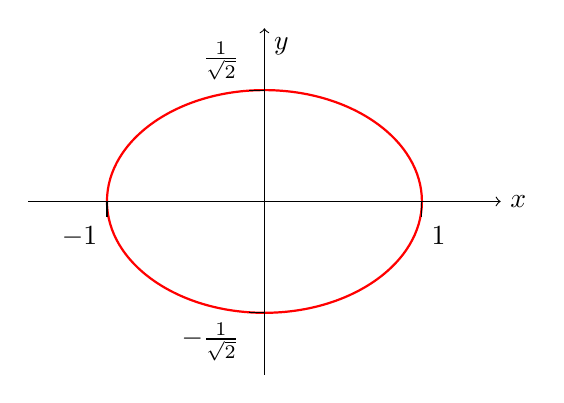
\begin{tikzpicture}[scale=2]
      \draw[thick,red,yscale={1/sqrt(2)}] (0,0) circle [radius=1];
      \draw[->] (-1.5,0) -- (1.5,0) node[right] {$x$};
      \draw[->] (0,-1.1) -- (0,1.1) node[below right] {$y$};
      \draw (-1,0) -- +(0,-.1) node[below left] {$-1$};
      \draw (1,0) -- +(0,-.1) node[below right] {$1$};
      \draw (0,{-1/sqrt(2)}) -- +(-.1,0) node[below left] {$-\frac{1}{\sqrt{2}}$};
      \draw (0,{1/sqrt(2)}) -- +(-.1,0) node[above left] {$\frac{1}{\sqrt{2}}$};
    \end{tikzpicture}
